%!TEX root = ../username.tex
\chapter{Real-time Audio Programming}
\hspace*{-0.15cm}This chapter will consider the theory behind real-time audio programming and the different principles that are followed to create a functional program. It will begin with an overview of digital signal processing. Specifically, this will include the mathematical background required to understand sound. Next, it will cover the methods by which a digital system communicates with several components to create sound. Specifically, this will include how audio data is handled by a digital system's drivers and its corresponding speakers. After, the requirements that a real-time audio program needs in order to function will be considered. This will include a program's typical structure and functionality. Finally, libraries and other software available that handles these requirements will be discussed in length - focusing primarily on the Virtual Studio Technology specification.

\section{Sound As a Discrete Signal}
Sound is a physical phenomenon. Vibrations travel though a medium such as air to create waves and differences in pressure, which travel at the the speed of sound (roughly 331 m/s) \cite{Ling_2016}. These vibrations have varying lengths and intensity depending on the manner in which the sound is created. Changes in frequency are reflected as the pitch of a tone, such as different notes on an instrument. Changes in intensity reflect how loud a particular sound is, such as the different dynamics one can play on an instrument \cite{Ling_2016}. The human brain interprets these differences in pressure by converting waves into electrical signals. When a wave reaches the human ear, the ear canal resonates and converts the sound into mechanical vibrations for the cochlea \cite{Ling_2016}. The cochlea in turn converts these into electrical signals for the brain. Like the human brain, interpreting sound in a digital setting involves simplifying the physical nature of sound waves into a format understandable by computers.

Consider Figure 3.1.

\begin{figure}[h] % [h] used to prevent {figure} from doing weird positioning
\begin{center}
	\fbox{
	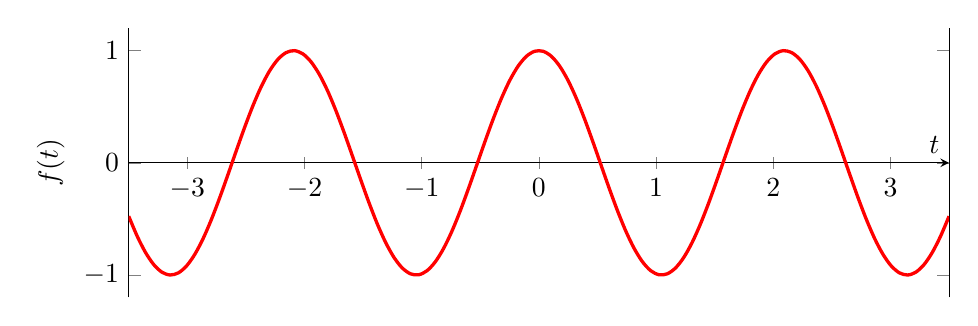
\begin{tikzpicture}
		\begin{axis} [
			axis x line = middle, % The x axis should go through the origin
			xlabel = \(t\),
			ylabel = {\(f(t)\)},
			height = 5cm,
			width = 12cm
			]

			\addplot [
			jump mark mid,
			domain = -3.5:3.5,
			samples = 100,
			smooth,
			very thick, red
			] {(cos(deg(3 * x)))};

		\end{axis}
	\end{tikzpicture}}
	\caption{A graph of the wave \(f(t) = cos(3t)\).}
\end{center}
\end{figure}

This is a representation of a sinusoid under the time domain. Each crest and trough represent the compressions and rarefactions that occur in real life when this tone is created. By graphing the sinusoid with respect to time, one can view the particular waveform that is created from this given sound. This is an example of a \textit{continuous sinusoidal signal}. They are defined by the following expression:

\begin{defn}[Definition of a continuous sinusoid]\label{def1}
	\begin{equation}\label{introf(t)}
	f(t)=Acos(2\pi ft + \varTheta), t \in (-\infty, \infty)
\end{equation}\end{defn}

where \textit{f} is frequency, \textit{t} is time, and $\varTheta$ is the phase offset in radians \cite{Symons_2013}. By taking the sum of several sinusoids, one can create (or deconstruct) any type of non-sinusoidal signal, given a sufficiently high number of sine waves are used. This is defined as:

\begin{defn}[Definition of a non-sinusoidal continuous signal]\label{def2}
	\begin{equation}\label{intro2f(t)}
	f(t)=\sum_{k=1}^{N_h} A_k cos(2\pi kft + \varTheta_k)
\end{equation}\end{defn}

where \textit{k} is one sinusoid in the sum, $N_h$ is the number of total sinusoids used to construct the signal, $A_k$ the amplitude of a particular signal for each \textit{k}, $\varTheta_k$ the phase for each \textit{k}, and \textit{f} the fundamental frequency of $f(t)$ \cite{Symons_2013}. With this definition in mind, any signal - and therefore, any sound - can be represented as the sum of several sinusoids, seen in Figure 3.2.

\begin{figure}[h] % [h] used to prevent {figure} from doing weird positioning
\begin{center}
	\fbox{
	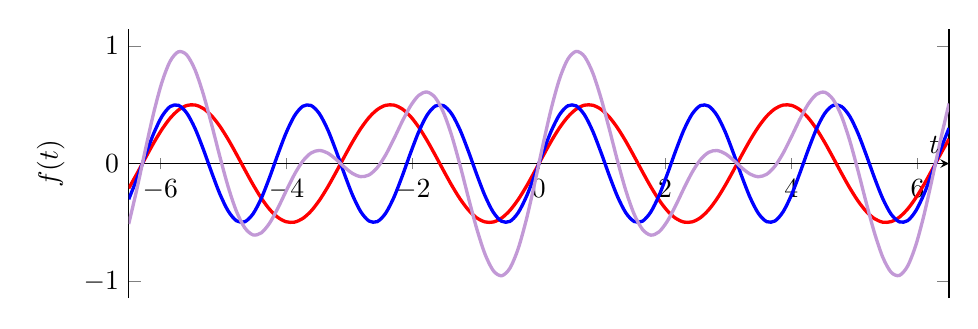
\begin{tikzpicture}
		\begin{axis} [
			axis x line = middle, % The x axis should go through the origin
			xlabel = \(t\),
			ylabel = {\(f(t)\)},
			height = 5cm,
			width = 12cm
			]

			\addplot [
			jump mark mid,
			domain=-6.5:6.5,
			samples=100,
			smooth,
			very thick, red
			] {(0.5 * sin(deg(2 * x)))};

			\addplot [
			jump mark mid,
			domain=-6.5:6.5,
			samples=100,
			smooth,
			very thick, blue
			] {(0.5 * sin(deg(3 * x)))};

			\addplot [
			jump mark mid,
			domain=-6.5:6.5,
			samples=100,
			smooth,
			very thick, blue!60!red!40 %xcolor the goat
			] {((0.5 * sin(deg(3 * x))) + (0.5 * (sin(deg(2 * x)))))};
		\end{axis}
	\end{tikzpicture}}
	\caption{A graph of a waveform, deconstructed to its sinusoids.}
\end{center}
\end{figure}

To create a digitial representation of this signal, the \textit{Nyquist-Shannon Sampling Theorem} provides guidelines for how signals should be \textit{bandlimited} - or rather, have their frequencies limited - and how often a signal should be sampled to ensure its accuracy.

\begin{defn}[The Nyquist-Shannon Sampling Theorem \cite{Orfanidis_1998}]\label{def3}
\hfill
\begin{enumerate}
	\item The signal must be \textit{bandlimited}, containing no frequencies beyond a particular maximum $F_{max}$.
	\item The \textit{sampling rate} of a signal must be at least twice the maximum frequency $F_{max}$.
\end{enumerate}
\end{defn}

The human ear provides sufficient guidelines for each of these requirements. Typical human hearing spans across a range of 20 Hz - 20,000 Hz \cite{Ling_2016}. As such, the \textit{Nyquist rate} - the minimum sampling rate - for a signal corresponding to an audio waveform must encompass this range. It is defined as $F_s = 2F_{max}$ \cite{Orfanidis_1998}. With an $F_{max} = 20,000$ Hz, the Nyquist rate for audio DSP applications is thus 40,000 Hz. This explains the sample rate for several audio applications. Modern audio recordings use 44,100 Hz, and Digital Audio Workstations usually produce with 48,000 Hz. With this Nyquist rate, the entire range of human hearing is covered.

The process of \textit{sampling} an analog signal is done by taking measurements of a particular function at regular points in time. Each individual measurement of the original analog signal is a \textit{sample}. By convention, samples are in the range (-1,1). This is in alignment with []. [talk about format of .wav files and how 16bit wav uses ints of various size etc. etc.]

\begin{figure}[h] % [h] used to prevent {figure} from doing weird positioning
	\begin{center}
		\fbox{
		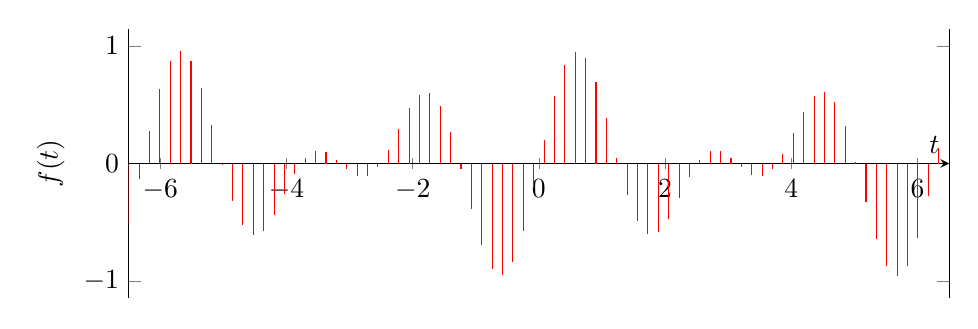
\begin{tikzpicture}
			\begin{axis} [
				axis x line = middle, % The x axis should go through the origin
				xlabel = \(t\),
				ylabel = {\(f(t)\)},
				height = 5cm,
				width = 12cm
				]

				\addplot+ [
				ycomb,
				mark = text,
				text mark = , % so jank
				domain = -6.5:6.5,
				samples = 80,
				red
				] {((0.5 * sin(deg(3 * x))) + (0.5 * (sin(deg(2 * x)))))};

			\end{axis}
		\end{tikzpicture}
		}
		\caption{A discrete graph of a waveform taken with 80 samples.}
	\end{center}
\end{figure}

This is a discrete representation of our original continuous signal. Such a snippet above represents a \textit{buffer} of data. Under this representation, one may predict how to represent this in code. If each sample refers to a \textit{float} in the range (-1,1), an array of floats is sufficient to store this waveform in memory. With this representation of sound, one can now use this data to process sound digitally.

\section{The Real-time Programming Bus Schedule}

In a digital system, hardware components get the attention of the processor by sending \textit{interrupts} \cite{Rubini2005-kv}. Keyboards, hard drives, and network cards are all components that use interrupts. By using interrupts, one can account for real-world imperfections in the transfer of data. Speakers, likewise, utilize interrupts for the playback of sound. To play sound, a continuous stream of audio data must be sent to the sound card or audio chipset of the device \cite{Walker_2005}. To do this, data is sent in chunks, each known as a \textit{buffer}. When the sound card finishes playing a buffer, it sends an interrupt to the processor requesting a new one for playback. For most applications, buffer sizes can be large enough to prevent audio from ever dropping. This allows for intermediate applications or virtual mixers to play audio from multiple sources without issue. However, in the case that lower latency is expected for the end user, shortening buffer sizes can do so at the cost of higher performance requirements \cite{corless2009pc-based}. This high performant expectation is an example of a \textit{real-time system}, which is defined as follows:

\begin{defn}[Definition of a Real-time System \cite{realtimefaq}]\label{def3}
\hfill \break
A real-time system is one in which the correctness of the computations not
only depends upon the logical correctness of the computation but also upon
the time at which the result is produced.

\begin{center}
\hspace*{-10.8cm}\textnormal{Extended for DSP applications:}
\end{center}

\hspace*{-0.6cm}In a real-time DSP process, the analyzed (input) and/or generated (output)
samples (whether they are grouped together in large segments or processed
individually) can be processed (or generated) continuously in the time it
takes to input and/or output the same set of samples independent of the
processing delay.

\end{defn}

Suppose, then, that a hardware device or software application interrupts the processor in the same manner during the time a high performant application is expected. To prevent low-priority interrupts from being executed before high-priority calls, \textit{preemption} allows the processor to prioritize interrupts to maintain correctness in a real-time system \cite{realtime-linux}. On UNIX-like operating systems, interrupts are queued to be executed by the processor with a priority number. They are then dequeued in priority order, thus allowing applications with real-time requirements the ability to be prioritized \cite{posix4}. While real-time systems can differ in how integral it is that deadlines are met, the audio stream can continue playback even if buffers are dropped. This is an example of a \textit{soft real-time system}, as deadlines only need to be maintained \textit{on average} \cite{realtime-linux}. In an ideal world, however, no buffers should be dropped to maintain integrity of the audio stream.

Consider Figure 3.4:

\begin{figure}[h] % [h] used to prevent {figure} from doing weird positioning
	\begin{center}
		\fbox{
		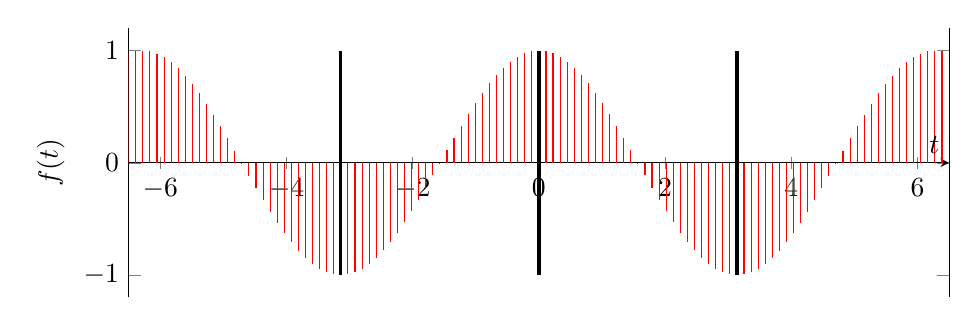
\begin{tikzpicture}
			\begin{axis} [
				axis x line = middle, % The x axis should go through the origin
				xlabel = \(t\),
				ylabel = {\(f(t)\)},
				height = 5cm,
				width = 12cm
				]

				\addplot+ [
				ycomb,
				mark = text,
				text mark = , % so jank
				domain = -6.5:0,
				samples = 59,
				red
				] {(cos(deg(x))};

				\addplot+ [
				ycomb,
				mark = text,
				text mark = , % so jank
				domain = 0:6.5,
				samples = 59,
				red
				] {(cos(deg(x))};

				\addplot+ [
				ycomb,
				very thick,
				mark = text,
				text mark = , % so jank
				domain = -6.5:6.5,
				samples = 80,
				black
				] coordinates {(3.141592, -1) (3.141592, 1)};

				\addplot+ [
				ycomb,
				very thick,
				mark = text,
				text mark = , % so jank
				domain = -6.5:6.5,
				samples = 80,
				black
				] coordinates {(-3.141592, -1) (-3.141592, 1)};

				\addplot+ [
				ycomb,
				very thick,
				mark = text,
				text mark = , % so jank
				domain = -6.5:6.5,
				samples = 80,
				black
				] coordinates {(0, -1) (0, 1)};

			\end{axis}
		\end{tikzpicture}
		}
		\caption{A discrete graph distinguishing buffers at regular intervals.}
	\end{center}
\end{figure}

If a buffer is dropped in the digital system, it cannot be output by the speaker. The resulting sound will ``click'' and ``pop'' where there is a gap in the audio stream \cite{Walker_2005}.

\begin{figure}[h] % [h] used to prevent {figure} from doing weird positioning
	\begin{center}
		\fbox{
		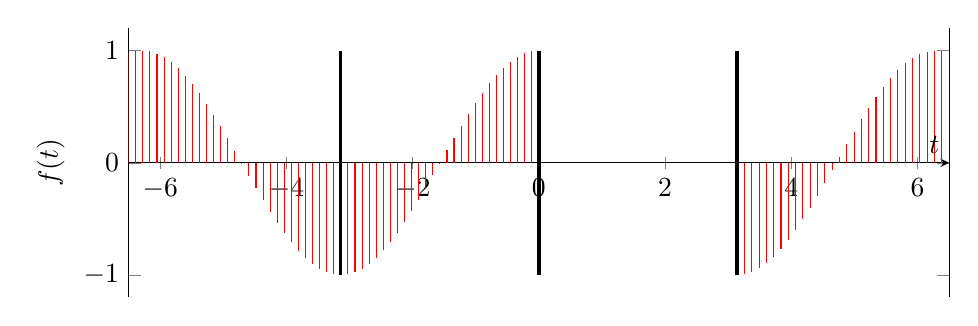
\begin{tikzpicture}
			\begin{axis} [
				axis x line = middle, % The x axis should go through the origin
				xlabel = \(t\),
				ylabel = {\(f(t)\)},
				height = 5cm,
				width = 12cm
				]

				\addplot+ [
				ycomb,
				mark = text,
				text mark = , % so jank
				domain = -6.5:0,
				samples = 59,
				red
				] {(cos(deg(x))};

				\addplot+ [
				ycomb,
				mark = text,
				text mark = , % so jank
				domain = 3.1415:6.5,
				samples = 30,
				red
				] {(cos(deg(x))};

				\addplot+ [
				ycomb,
				very thick,
				mark = text,
				text mark = , % so jank
				domain = -6.5:6.5,
				samples = 80,
				black
				] coordinates {(3.141592, -1) (3.141592, 1)};

				\addplot+ [
				ycomb,
				very thick,
				mark = text,
				text mark = , % so jank
				domain = -6.5:6.5,
				samples = 80,
				black
				] coordinates {(-3.141592, -1) (-3.141592, 1)};

				\addplot+ [
				ycomb,
				very thick,
				mark = text,
				text mark = , % so jank
				domain = -6.5:6.5,
				samples = 80,
				black
				] coordinates {(0, -1) (0, 1)};

			\end{axis}
		\end{tikzpicture}
		}
		\caption{A discrete graph with a dropped buffer.}
	\end{center}
\end{figure}

To prevent this from occuring, processing must occur within the time it takes to output a single buffer. The maximum time to process buffers is dependent of the buffer size. Suppose a single buffer is measured by an amount, \textit{x}, which corresponds to the number of samples present in a single buffer of audio data. To obtain the amount of time \textit{t} that a digital system would take to output this buffer, \textit{x} can be divided by the \textit{sample rate}, measured in Hz. This measurement of Hz is by definition the reciprocal second. Thus, dividing the buffer size by the sample rate provides the time in seconds that the buffer takes to be output. For a buffer size \textit{x} of 256 samples and a \textit{sample rate} of 48,000 Hz, the resulting time \textit{t} would be $(256 / 48,000)$, or 0.0053 seconds. Any such program working with real-time audio must compute a buffer during this time frame. Should processing take too long, audio will be dropped as seen in Figure 3.5.

To summarize, Figure 3.6 describes how this data travels in a digital setting.

\begin{figure}[h] % [h] used to prevent {figure} from doing weird positioning
	\tikzstyle{startstop} = [rectangle, minimum width=3cm, minimum height=1cm,text centered, align=center, draw=black]
	\tikzstyle{arrow} = [thick,->,>=stealth]
	\begin{center}
		\fbox{
		\begin{tikzpicture}
			\node (start) [startstop] {Speakers, Microphones, etc. \\
				\begin{tikzpicture}
					\node (start) [startstop] {DAC};
				\end{tikzpicture}
				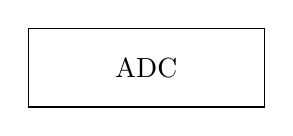
\begin{tikzpicture}
				\node (A) [startstop] {ADC};
				\end{tikzpicture}
			};
			\node (A) [startstop, right of=start, xshift=5cm] {Sound Card \\
			(Generally Integrated)};
			\node (B) [startstop, right of=A, xshift=4cm] {Driver};
			\node (C) [startstop, below of=B, yshift=-1.3cm] {OS \\
			(Win, Mac, etc.)};
			\node (D) [startstop, left of=C, xshift=-4cm] {Audio Driver \\
			(ASIO, JACK, etc.)};
			\node (end) [startstop, left of =D, xshift=-5cm] {Host Application \\
				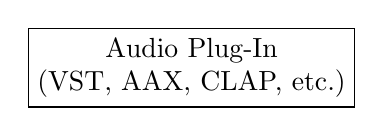
\begin{tikzpicture}
					\node (start) [startstop] {Audio Plug-In \\
					(VST, AAX, CLAP, etc.)};
				\end{tikzpicture}
			};

			\draw [<->, thick] (start) ++(3.2, 0) -- +(0.58, 0);
			\draw [<->, thick] (A) -- node {} (B);
			\draw [<->, thick] (B) -- node {} (C);
			\draw [<->, thick] (C) -- node {} (D);
			\draw [<->, thick] (D) ++(-3.55, 0) -- +(1.69, 0);
		\end{tikzpicture}
		}
		\caption{The flow of information for audio data in a digital system.}
	\end{center}
\end{figure}

Audio is first processed by the audio plugin under a particular host application. This host application handles several different audio plugins to generate and manipulate sound. This audio is then processed by the audio driver into buffers. Buffers are stored in memory until the processor is interrupted by the audio chipset or sound card, upon which the buffer is sent to be output to the system's speakers. This is completed by the Digital-to-Analog Converter (DAC) which converts the discrete signal into a continuous form for the speaker.

A real-time program does not play audio files akin to one using sound effects for a video game; the program needs to play this sound as it is being generated on-the-fly. As one can imagine, this will provide limitations into the implementation of the program to prevent buffers from being dropped.

%\section{Discrete Signals Applied}

\section{Program Structure \& Libraries}
The typical structure of an audio program separates the internal processing and the external GUI into multiple threads. The audio thread typically runs at a speed determined by the host application it runs under, often times configurable in the settings. Each buffer sent []. The GUI runs at a much lower speed [reword to be more rigorous] and communicates to the audio thread via signals (note that this is different to the audio signal being sent to the sound card). This type of structure is more generally known as a \textit{Model View Controller} design pattern. Specifically, a variation of this model is used that combines the view and controller of the model \cite{Bucanek2009}. Figure 3.7 provides a diagram of this.

\begin{figure}[h] % [h] used to prevent {figure} from doing weird positioning
	\tikzstyle{startstop} = [rectangle, minimum width=3cm, minimum height=1cm,text centered, align=center, draw=black]
	\tikzstyle{arrow} = [thick,->,>=stealth]
	\begin{center}
		\fbox{
		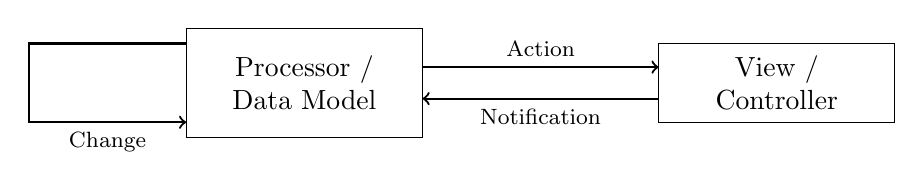
\begin{tikzpicture}
			\node (start) [inner sep=10pt, startstop] {Processor / \\ Data Model};
			\node (A) [startstop, right of=start, xshift=5cm] {View / \\  Controller};

			\draw [->, thick] (start) ++(1.5, 0.2) -- node[anchor=south] {\footnotesize{Action}} +(3, 0) (A);
			\draw [<-, thick] (start) ++(1.5, -0.2) -- node[anchor=north] {\footnotesize{Notification}} +(3, 0) (A);
			\draw [->, thick] (start) ++(-1.5,0.5) -- +(-2,0) -- +(-2,-1) -- node[anchor=north] {\footnotesize{Change}} +(0, -1) (start);
		\end{tikzpicture}
		}
		\caption{A Model of an Audio Plugin Application.}
	\end{center}
\end{figure}

This alone can provide the higher-level structure to a UML diagram. If one were to separate the processing and view of a particular application, this could be done by separating the processing and GUI into two distinct classes:

[insert UML diagram here with just two things ig]

\begin{figure}[h]
	\begin{center}
		\fbox{\includegraphics{example.1}}
		\caption{UML Diagram of an audio application.}
	\end{center}
\end{figure}

For the purposes of this thesis, [].

%\lstset{language =[ANSI]C++}
%\lstset{backgroundcolor=\color{white},rulecolor=\color{black}}
%\lstset{linewidth=.95\textwidth,breaklines=true}
%\lstset{commentstyle=\textit,stringstyle=\upshape,showspaces=false}
%\lstset{frame = single}
%\lstset{numbers=left,numberstyle=\tiny,basicstyle=\small}
%\lstset{commentstyle=\normalfont\itshape,breakautoindent=true}
%\lstset{abovecaptionskip=1.2\baselineskip,xleftmargin=30pt}
%\lstset{framesep=6pt}
%\begin{singlespace}
%\lstinputlisting[caption=VST3 Project Generator Script Usage, label=motion]{source/template.txt}
%\end{singlespace}

With the design of the plugin taken care of, one can begin implementation of the plugin processor that will manipulate the input signal.
